\documentclass[10pt]{article}\usepackage[margin=.65in]{geometry}\usepackage[T1]{fontenc}\usepackage{graphicx}\setlength{\parindent}{0pt}\setlength{\parskip}{7pt}\sloppy\begin{document}{\large Stored validity test correspondence}\par 5 main declarations and 7 fixed controls compiled, with 12 separate named axiom readbacks. This packet archives completed producer evidence; independent review is pending.\par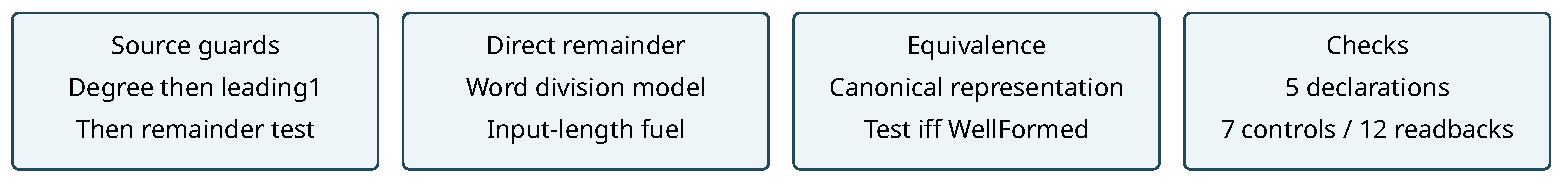
\includegraphics[width=\linewidth]{diagram.pdf}\par Construction. The source-ordered test checks degree, then the active leading word, then emptiness of the residual remainder. The proof uses FallbackGeometry.remainder and its word-division model directly with input-length fuel. Successful testing is equivalent to StoredInput.WellFormed under the representation premises; residual divisibility is derived rather than assumed. Degree guard safety precedes indexing.

Assumptions and boundary. The domain is prime 1$<$p$<$2\textasciicircum{}31, canonical polynomial coefficients, capacities three/two and canonical coefficients in every stored slot. Native odd-field validation admits p$>$=5; the helper domain is broader. A boundary control shows the native-style test can accept noncanonical inactive padding: canonical storage is an external premise, not a validator guarantee. The correspondence covers n=1/no tables and modeled values, not physical memory or compiler behavior.

Evidence. All successful receipts report unchanged bound inputs. The false theorem was rejected with exit one. Named readbacks contain only permitted foundational axioms. Exact sources, source snapshots, commands and failed attempts are under producer. Compiler and dependency caches were reused and hash-bound; no independent binary rechecker or transient-edit exclusion is claimed.

Retained failures and next work. Three failed development attempts are retained. The false theorem and three malformed-inventory controls were rejected. Independent source-fidelity review and the separate dispatch-to-test corollary remain pending.

Sources. The immutable native three\_leads.rs snapshot and dependency inventories are retained in producer, alongside the original detailed report. This composes existing source and polynomial proofs and makes no new-method claim. The graph shows proof structure because there are no comparative measurements. No scientific trajectory, cost ratio, runtime admission or campaign limit changed.
\end{document}